\chapter{Determining Reachability using Weak and Strong Attractors}
\mytodo{formal problem statement}
In this section, we introduce an algorithm for computing AS-reachability. It is based on the notion of strong- and weak-attractors by Hahn et\ al. \cite{chaudhuri_simple_2016}. In the context of AS-reachability, it is not necessary to consider the precise probabilities of a particular transition; knowing whether the probability of the transition is non-zero suffices. It is also useful to introduce an additional ``nature'' player, that replaces the probabilistic choices. This leads us to define a new model, equivalent in terms of AS-reachability, for two-player games:
\begin{mydefinition}{Reachability Game with Nature (RGN)}{def:rgn}
Let $\mathcal{G} = (\set{0, 1}, S, A, \set{S_0, S_1}, \Delta, AP, \chi)$ be a two-player SMG.

The equivalent \textit{reachability game with nature} is a tuple $\mathcal{P}=(S_0, S_1, S_N, E)$ with\begin{itemize}
    \item the state set of the nature player $S_N\defeq\set{(s,a)\in S\times A\mid\Delta(s, a)\neq\bot}$
    \item and a transition relation $E\defeq\set{(s, (s, a))\in S\times S_N}\cup\\
    \set{((s,a), s')\in S_N\times S\mid\Delta(s, a)(s')>0}$
\end{itemize}
\end{mydefinition}
The \textit{predecessors} of a set of states $T$ are defined as $\Pred(T) \defeq \set{s' \in S \mid (s', s) \in E, s \in T }$, and the \textit{successors} are defined as $ \Succ(T) \defeq \set{s' \in S \mid (s, s') \in E, s \in T }$. For a single state, set braces may be omitted: $\Pred(s) \defeq \Pred(\set{s})$. Furthermore, we use the following notation to remove a set of states $A$ from a RGN:\\$\mathcal{P}\setminus B\defeq (S_0\setminus B,\ S_1\setminus B,\ S_N\setminus B,\ \set{(s, s')\in E\mid s,s'\notin B})$.

A path $s_0(s_0, a_0)s_1(s_1, a_1)\dots$ of an RGN corresponds to the path $s_0a_0s_1a_1\dots$ in the original SMG. To simplify notation, we use the latter form for RGNs as well. Using this path notation, we can define strategies for RGNs identically to SMGs (see section \ref{def:strat}).

\begin{myexample}{Simple RGN}{exmp:simple_rgn}
Figure~\ref{fig:example_game_01_rgn} shows an example of a RGN. It is a translation of the SMG shown in figure~\ref{fig:example_game_01} with the player's \textit{triangle} and \textit{circle} forming a coalition. The probabilistic choices are represented by labeled states. For example, the probability distribution $\Delta(s_1, a)$ was replaced by the nature state $(s_1, a)$ with outgoing edges to states that have a non-zero probability under $\Delta(s_1, a)$. The exact values of these probabilities are irrelevant for the RGN. 
\end{myexample}

\begin{figure}[t]
\centering
\begin{tikzpicture}[>=stealth, node distance=3cm, every node/.style={font=\small}]
    % Nodes
    \node[draw, minimum size=1cm, shape=rectangle] (S1) {$\textcolor{myred}{s_1}$};
    \node[draw, minimum size=1cm, shape=circle,right= 5cm of S1] (S2) {$\textcolor{mypink}{s_2}$};
    \node[draw, minimum size=1cm, shape=circle, below= 3cm of $(S1)!0.5!(S2)$] (S3) {$s_3$};
    \draw[-] (S1) -- node[below left, pos=0.5] {} ($(S1)!0.5!(S3)$);
    \filldraw[black] ($(S1)!0.5!(S3)$) circle (2pt) 
        node[label={225:$\textcolor{myblue}{(s_1,a)}$}] {}; % Labeled dot at split point
        
    \draw[->] ($(S1)!0.5!(S3)$) -- node[below left, pos=0.5] {} (S3);
    \draw[->] ($(S1)!0.5!(S3)$) -> node[below, pos=0.75] {} (S2);
    \draw[-] (S2) -- node[below right, pos=0.5] {} ($(S2)!0.5!(S3)$);
    \filldraw[black] ($(S2)!0.5!(S3)$) circle (2pt) 
        node[label={315:$\textcolor{myblue}{(s_2,a)}$}] {}; % Labeled dot at split point
        
    \draw[->] ($(S2)!0.5!(S3)$) -- node[below right, pos=0.5] {} (S3);
    \draw[->] ($(S2)!0.5!(S3)$) -- node[below, pos=0.75] {} (S1);
    \draw[->] (S1) to[bend left=30] node[above, pos=0.25] {} 
    node[above, pos=0.75] {} coordinate[pos=0.5] (S1S2) (S2);
    \filldraw[black] (S1S2) circle (2pt) 
        node[label={90:$\textcolor{myorange}{(s_1, b)}$}] {}; % Labeled dot halfway along the curve
        
    \draw[->] (S2) -> node[above, pos=0.25] {} node[above, pos=0.75] {} coordinate[pos=0.5] (S2S1) (S1);
    \filldraw[black] (S2S1) circle (2pt) 
        node[label={270:$\textcolor{mygreen}{(s_2, b)}$}] {}; % Labeled dot halfway along the curve
        
    \draw[->] (S3) edge[loop below]
    coordinate[pos=0.5] (S3S3)
    node[right, pos=0.2] {}
    node[left, pos=0.8] {} (S3);
    \filldraw[black] (S3S3) circle (2pt) 
        node[label=270:{$\textcolor{myblue}{(s_3, c)}$}] {}; % Labeled dot halfway along the curve
        
\end{tikzpicture}
\caption{Translation of the SMG from figure~\ref{fig:example_game_01} into a RGN. The players represented by the circle and triangle nodes have been combined into a coalition.}
\label{fig:example_game_01_rgn}
\end{figure}



\section{Strong Attractors}\label{sec:satr}
Let $\mathcal{P}=(S_0, S_1, S_N, E)$ be a RGN. To understand AS-reachability in RGNs, it can be helpful to imagine the current state as a ``pebble'' on the game graph, with players moving this pebble across states according to their strategies. We consider the set of pebble positions (states) from which a player $i\in\set{0, 1}$ can force the pebbles into a target set $T\subseteq S$ with cooperation of the nature player. This set is called the \textit{strong attractor} of $T$, denoted $\satr_i(T, \mathcal{P})$. And we will see that this corresponds to those states from which the player can reach the target set with a non-zero probability in the original game $T$.


To compute \( \satr_i(T, \mathcal{P}) \), we use a fix-point calculation. Starting with the target set \( T \), we iteratively look at each predecessor state $s$ of the current working set and add it if it meets the following conditions:
\begin{enumerate}
    \item\( s \) belongs to player \( i \) or the nature player (\( s\in S_i \cup S_N \)), or
    \item\( s \) belongs to the opposing player (\( s\in S_{1-i} \)), and all successor states of \( s \) are already in the working set.
\end{enumerate}

Formally, we compute a sequence of sets $(A_k)_{k\in\N}$ with:
\begin{alignat*}{2}
    A_0 &\defeq T\\
    A_{k+1} &\defeq A_k&&\cup\set{s\in S_i\cup S_N\mid \exists s'\in A_k: (s, s')\in E}\\
    & &&\cup\set{s\in S_{1-i}\mid\forall (s, s')\in E: s'\in A_k}\\
    &= A_k&&\cup\set{s\in \Pred(A_k)\mid s\in S_i\cup S_N\text{ or } \Succ(s)\subseteq A_k}
\end{alignat*}  
\mytodo{this is only correct if every state has a successor}
The strong attractor for player $i$ of $T$ is then given by:\[
    \satr_i(T, \mathcal{P}) = \bigcup_{k\in\N} A_k
    \]
\begin{myproposition}{Strong Attractors Compute Reachability}{prop:reach}\label{prop:reach}
    Let $\mathcal{G} = (\set{0, 1}, S, A, \set{S_0, S_1}, \Delta, AP, \chi)$ be a two-player SMG and\\
    $\mathcal{P}=(S_0, S_1, S_N, E)$ be the corresponding RGN. It holds that:\[
        \satr_i(T, \mathcal{P})\cap S = \Reach_i(T, \mathcal{G})\hspace{1.5cm}i\in\set{0, 1}
        \]
\end{myproposition}

\begin{proof}
    We first show that $\satr_i(T, \mathcal{P})\cap S \subseteq \Reach_i(T, \mathcal{G})$ by induction:
    
    Every state $s\in\satr_i(T, \mathcal{P})\cap S_i$ is either in $T$ or there is a $k\in\N$, s.t. $s\in A_{k+1}$, $s\notin A_k$. Let $(s, a_s)\in S_N\cap A_k$ denote a successor state of $s$ in $A_k$. There is such a state, as all successor states of $s$ belong to the nature player $S_N$. For any prefix $\lambda\in (SA)^\ast$, we define a strategy $\sigma_i$ for player $i$ as follows:\[
        \sigma_i(\lambda s)\defeq\begin{cases}
            \delta_{a_s} & \text{ if } s\in\satr_i(T, \mathcal{P})\\
            \delta_a\;\text{ for some } a\in A(s) & \text{ otherwise }
        \end{cases}
        \]
    And let $\sigma_{1-i}$ be an arbitrary strategy for the other player.
    
    It trivially holds that:\[
        \Pr_s^{(\sigma_0, \sigma_1)}(\Reach(T))>0 \;\text{ for } s\in T
    \]
    Let $k\in\N$ and $P_s^{(\sigma_0, \sigma_1)}(\Reach(T))>0$ for all $s\in A_j\cap S, j\leq k$. For all $s'\in A_{k+1}\cap S$ it holds that, if
    \begin{description}
        \item[Case 1: $s'\in S_i$.] 
         Then $\sigma_i(s')=\delta_{a_{s'}}$. This means player $i$ chooses the action $a_{s'}$ according to his strategy $\sigma_i$. As $(s', a_{s'})\in A_k$ and $(s', a_{s'})\notin T$, it has a successor $s''\in A_k$ and as $(s', a_{s'})\in S_N$, it holds that $\Delta(s', a_{s'})(s'')>0$.
        \item[Case 2: $s'\in S_{1-i}$.]
        Let $\sigma_{1-i}(s')$ be any distribution over $A(s')$ and let $a\in A$ be an action with $\sigma_{1-i}(s')(a)>0$. As all successors of $s'$ are in $A_k$, it holds that $(s', a)\in A_k$. Analogously to above, it follows: $P_{s'}^{(\sigma_0, \sigma_1)}(\Reach(T))>0$.
    \end{description}
    We can deduce inductively that $\satr_i(T, \mathcal{P})\cap S \subseteq \Reach_i(T, \mathcal{G})$.
    
    Now, to show the other inclusion, let $s\in S\setminus\satr_i(T, \mathcal{P})$. There exists no $k\in\N$ with $s\in A_k$. This also means that if
    \begin{description}
        \item[Case 1:] $s$ belongs to player $i$, then $\Succ(s)\cap\satr_i(T, \mathcal{P})=\emptyset$ or if
        \item[Case 2:] $s$ belongs to player $1-i$, then $\Succ(s)\cap(S_N\setminus\satr_i(T, \mathcal{P}))\neq\emptyset$.
    \end{description}
    Let  $(s, a_s)\in S_N\setminus\satr_i(T, \mathcal{P})$ denote a successor of $s$. For any prefix $\lambda\in (SA)^\ast$, we define a strategy for player $1-i$:
    \[
        \sigma_{1-i}(\lambda s)\defeq\begin{cases}
            \delta_{a_s} & \text{ if } s\notin\satr_i(T, \mathcal{P})\\
            \delta_a\;\text{ for some } a\in A(s) & \text{ otherwise }
        \end{cases}
    \]
    Let $\sigma_i$ be an arbitrary strategy of player $i$. If
    \begin{description}
        \item[Case 1: $s\in S_i$], then any following state with a non-zero probability under $\sigma_i$ has to be outside of $\satr_i(T, \mathcal{P})$, as $s$ has no successors in $\satr_i(T, \mathcal{P})$ and any nature state outside of $\satr_i(T, \mathcal{P})$ also has no successors in $\satr_i(T, \mathcal{P})$.
        \item[Case 2: $s\in S_{1-i}$], then according to the definition of $\sigma_{1-i}$, any following state with a non-zero probability under $\sigma_{i-1}$ is outside of $\satr_i(T, \mathcal{P})$.
    \end{description}
    Therefore $P_{s}^{(\sigma_0, \sigma_1)}(\Reach(\satr_i(T, \mathcal{P})))=0$ and as $T\subseteq\satr_i(T, \mathcal{P})$, it also holds that $P_{s}^{(\sigma_0, \sigma_1)}(\Reach(T))=0$. Thus $S\cap\Reach_i(T, \mathcal{G}) \subseteq \satr_i(T, \mathcal{P})$.
    
\end{proof}
\begin{mylemma}{Memoryless Strategy for Reachability}{lem:memless_satr}\label{lem:memless_satr}
There is a memoryless strategy for player $i$ reach a target set $T$ with a non-zero probability.
\end{mylemma}
\begin{proof}
The strategy constructed in the proof for proposition \ref{prop:reach} is memoryless.
\end{proof}

\begin{myexample}{Strong Attractors}{exmpl:satr}
Let $\mathcal{P}=(\set{s_1}, \set{s_2, s_3}, \set{(s_1, a), (s_1, b), (s_2, a), (s_2, b), (s_3, c)}, E)$ be the RGN shown in figure~\ref{fig:example_game_01_rgn}, with the square nodes representing player $0$ and the circular nodes representing player $1$. The strong attractor of $T\defeq\set{s_3}$ for player $0$, $\satr_0(\set{s_3}, \mathcal{P})$, can be computed as follows:
\begin{align*}
    A_0 &=\set{s_3}\\
    A_1 &=\set{s_3, \textcolor{myblue}{(s_1, a), (s_2, a), (s_3, c)}}\\
    A_2 &=\set{s_3, (s_1, a), (s_2, a), (s_3, c), \textcolor{myred}{s_1}}\\
    A_3 &=\set{s_3, (s_1, a), (s_2, a), (s_3, c), s_1, \textcolor{mygreen}{(s_2, b)}}\\
    A_4 &=\set{s_3, (s_1, a), (s_2, a), (s_3, c), s_1, (s_2, b), \textcolor{mypink}{s_2}}\\
    A_5 &=\set{s_3, (s_1, a), (s_2, a), (s_3, c), s_1, (s_2, b), s_2, \textcolor{myorange}{(s_1, b)}}\\
    A_k &=A_5\quad\text{for }k\geq 5\\
\satr_0(\set{s_3}, \mathcal{P})&=\set{s_3, (s_1, a), (s_2, c), (s_3, c), s_1, (s_2, b), s_2, (s_1, b)}
\end{align*}
Note that $s_2$ was not added to $A_2$ even though it's a predecessor of $(s_2, a)$. This is because it belongs to the adversarial player and has another successor ($(s_2, b)$) that is not in $A_1$. After $(s_2, b)$ is added to $A_3$, $s_2$ gets included in $A_4$, because then all successors of $s_2$ are in $A_3$.
\end{myexample}
This example also shows that nature states and non-nature states are added in alternate iterations. We later use this fact in algorithm~\ref{alg:satr}, where two steps are calculated in one iteration. 


\section{Weak Attractors}\label{sec:watr}
Using a procedure to compute strong attractors, we can determine the set of \textit{weak attractors} of a target set \( T \). We will later show that this is identical to computing AS-reachability. Let the definitions be as above\mytodo{more precise}, with \( k \in \mathbb{N} \), and let \( (B_k)_{k \in \mathbb{N}}, (C_k)_{k \in \mathbb{N}} \) be sequences of state sets. We compute \( B_k \) and \( C_k \) as follows:
\begin{align*}
B_0 &\defeq\satr_i(T, \mathcal{P})\\
C_k &\defeq\satr_{1-i}(S\setminus B_k, \mathcal{P}\setminus T)\\
B_{k+1} &\defeq\satr_i(T, \mathcal{P}\setminus C_k)
\end{align*}
The weak attractor for player $i$ of $T$ then is given by:
\[
\watr_i(T,\mathcal{P}) =\bigcap_{k\in\N}B_k
\]
The intuition behind this is as follows: In any iteration \( k \), from any state \( s \), whenever a state outside the current working set \( B_k \) is reachable for the adversarial player, the target set cannot be AS-reachable from \( s \), so we remove \( s \) from the graph for the next iteration (\( \mathcal{P} \setminus C_k \)). Eventually, the working set will only contain states for which the adversarial player has no strategy to leave the set. This means we can choose a strategy such that the weak attractors are never left and there is a non-zero probability of reaching \( T \). Under such a strategy, the path might follow cycles inside the weak attractors that don't include a state of \( T \), but as these cycles must have a probability smaller than 1 (otherwise \( T \) wouldn't be reachable), the probability of not reaching \( T \) is 0. Therefore, the probability of reaching \( T \) is 1.

Figure~\ref{fig:ill:watr} illustrates the principle of weak attractors. In the first iteration, the strong attractor of $T$, $B_0$, was computed. But there is a set of states $C_0$ intersecting $B_0$ from which player $i$ has a strategy to reach $T$, but also player $1-i$ has a strategy for leaving the set $B_0$. By computing $B_1$, we remove the states $B_0\setminus B_1$, from which player $i$ can not enforce reaching $T$ without visiting $C_0$.


\begin{figure}[t]
    \centering
    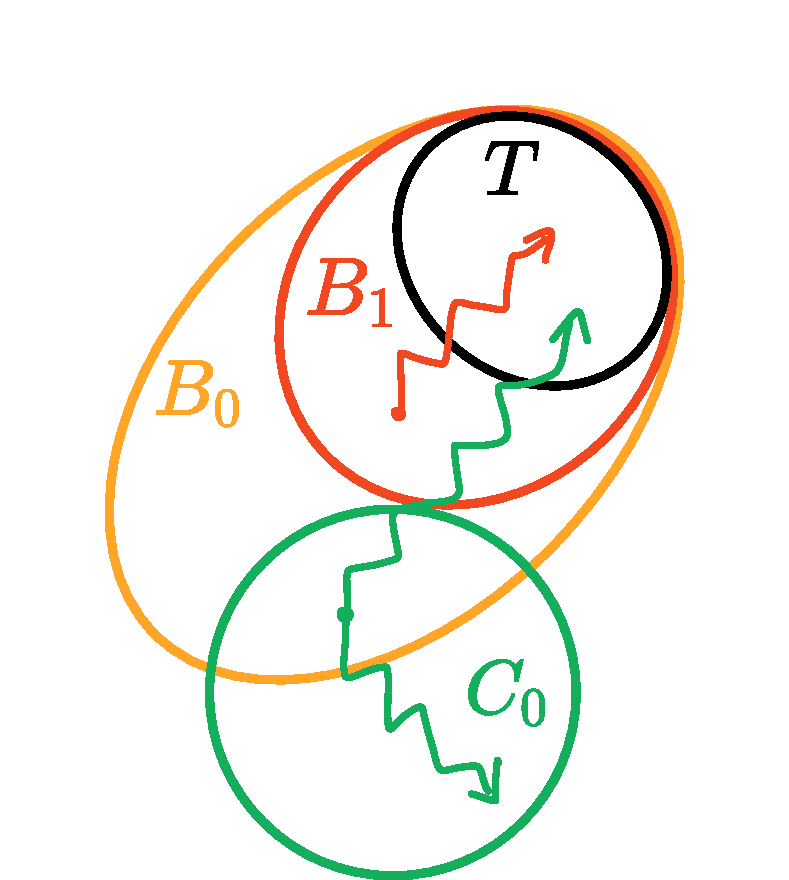
\includegraphics[width=0.5\linewidth]{figures/watr_illustration.pdf}
    \caption{Illustration showing the construction of weak attractors. In the area $B_0\setminus B_1$ player $i$ cannot enforce reaching $T$ without visiting $C_0$.}
    \label{fig:ill:watr}
\end{figure}

\begin{myproposition}{Weak Attractors Compute AS-Reachability}{prop:asreach}\label{prop:asreach}
    Let $\mathcal{G} = (\set{0, 1}, S, A, \set{S_0, S_1}, \Delta, AP, \chi)$ be a two-player SMG and\\
    $\mathcal{P}=(S_0, S_1, S_N, E)$ be the corresponding RGN. It holds that:\[
        \watr_i(T, \mathcal{P})\cap S = \ASReach_i(T, \mathcal{G})\hspace{1.5cm}i\in\set{0, 1}
        \]
\end{myproposition}
    

    
\begin{proof}
To prove proposition~\ref{prop:asreach}, we will begin by showing a few helpful statements. First, observe that for all $k\in\N$:
\begin{align}
B_{k+1}\cap S\subseteq B_k\cap S \text{ and } C_{k+1}\cap S\supseteq C_k\cap S. \label{eq:mono_B_k_C_k}
\end{align}
We show this by induction over $k$: For $k=0$, it holds that $B_1\cap S = \Reach_i(T, \mathcal{G}\setminus C_0)$. Any strategy used by player $1$ to reach $T$ in the game $\mathcal{G}\setminus C_0$ also works in the larger game $\mathcal{G}$. Otherwise, there would need to be a state $s\in\mathcal{G}\setminus C_0$ belonging to player $1-i$, from which they can force the play out of $\mathcal{G}\setminus C_k$, but such a state would be in $\Reach_{1-i}(S\setminus B_0, \mathcal{G}\setminus T)=C_0\cap S$ and thus not in $\mathcal{G}\setminus C_0$. Therefore, it holds that $B_{1}\cap S\subseteq B_0\cap S$.

Furthermore, $\Reach_{1-i}(S\setminus B_1, \mathcal{G}\setminus T) = C_1\cap S\supseteq C_0\cap S = \Reach_{1-i}(S\setminus B_0, \mathcal{G}\setminus T)$, as $S\setminus B_1\supseteq S\setminus B_0$.

Now let equation~\ref{eq:mono_B_k_C_k} hold for a $k\in\N$. With the same reasoning as above, any strategy used by player $1$ to reach $T$ in the game $\mathcal{G}\setminus C_{k+1}$ also works in the larger game $\mathcal{G}\setminus C_{k}$. Thus $B_{k+1}\cap S = \Reach_i(T, \mathcal{G}\setminus C_k)\subseteq \Reach_i(T, \mathcal{G}\setminus C_{k-1})=B_{k}\cap S$.

Similarly to above, it also holds that: $\Reach_{1-i}(S\setminus B_{k+1}, \mathcal{G}\setminus T) = C_{k+1}\cap S\supseteq C_k\cap S = \Reach_{1-i}(S\setminus B_k, \mathcal{G}\setminus T)$, as $S\setminus B_{k+1}\supseteq S\setminus B_k$. Thus, equation~\ref{eq:mono_B_k_C_k} holds by induction.

Because of this, we can choose an $l\in\N$, such that $B_l\cap S = B_{l+1}\cap S$ and $C_l\cap S = C_{l+1}\cap S$ (such an $l$ exists because $S$ is finite). It holds by the definition of $\watr_i$ that
\begin{align}
\watr_i(T, \mathcal{P})\cap S&\stackrel{\ref{eq:mono_B_k_C_k}}{=}B_l\cap S\nonumber\\
&=\satr_i(T, \mathcal{P}\setminus C_l)\cap S\nonumber\\
&\stackrel{\ref{prop:reach}}{=}\Reach_i(T, \mathcal{G}\setminus C_l)\label{eq:satr_l}
\intertext{and}
C_l\cap S &= \satr_{1-i}(S\setminus B_l, \mathcal{P}\setminus T)\cap S\nonumber\\
&\stackrel{\ref{prop:reach}}{=} \Reach_{1-i}(S\setminus B_l, \mathcal{G}\setminus T)\nonumber\\
&= \Reach_{1-i}(S\setminus \watr_i(T, \mathcal{P}), \mathcal{G}\setminus T).\label{eq:C_l}
\end{align}

To show \say{$\subseteq$} of proposition~\ref{prop:asreach}, let $s\in\watr_i(T, \mathcal{P})$. By equation~\ref{eq:satr_l}, there is an $l\in\N$ such that $s\in\Reach_i(T, \mathcal{G}\setminus C_l)$. Let $\sigma_i^\ast$ be the corresponding strategy of player $i$ to reach $T$ in the game $\mathcal{G}\setminus C_l$, and let $\sigma_{1-i}$ be an arbitrary strategy. It holds that $\Pr_s^{(\sigma_0^\ast, \sigma_1)}(\Reach(T)) > 0$. For the sake of contradiction, assume that for all $\sigma_i$ it holds that $\Pr_s^{(\sigma_0, \sigma_1)}(\Reach(T))< 1$. This means either there is a strategy $\sigma_{1-i}$, such that the play leaves $\watr_i(T, \mathcal{P})$ without visiting $T$ with a positive probability (case 1), or the play stays in $\watr_i(T, \mathcal{P})\setminus T$ indefinitely with a positive probability (case 2).

\begin{description}
    \item[Case 1:] It holds that $\forall\sigma_i\exists\sigma_{1-i}:\Pr_s^{(\sigma_0, \sigma_1)}(\Reach(S\setminus\watr_i(T, \mathcal{P}))\cap (S\setminus T)^\omega) > 0$. By determinacy (see theorem~\ref{theo:reach_det})\mytodo{introduce $\omega$ regular properties, state that they are measurable, and unions/intersections are also $\omega$ regular. State determinancy in terms of $\omega$-regular properties} the player $1-i$ has a strategy $\sigma_{1-i}'$ such that $\forall\sigma_i: \Pr_s^{(\sigma_0, \sigma_1)}(\Reach(S\setminus\watr_i(T, \mathcal{P}))\cap (S\setminus T)^\omega) > 0$ and therefore $s\in C_l\cap S\stackrel{\ref{eq:C_l}}{=}\Reach_{1-i}(S\setminus \watr_i(T, \mathcal{P}), \mathcal{G}\setminus T)$, which is a contradiction to $s\in\Reach_i(T, \mathcal{G}\setminus C_l)$.
    

    \item[Case 2:] In this case, let $W\coloneqq\watr_i(T,\mathcal{P})\setminus T$ and let $P\coloneqq (WA)^\omega$ denote the set of paths that always stay in $W$. It holds that $\forall\sigma_i\exists\sigma_{1-i}: \Pr_s^{(\sigma_0, \sigma_1)}(P) > 0$.
    
    Observe that for any $s'\in W$ it cannot hold, that a state inside $W$ is visited twice with probability $1$:\[
    \forall\sigma_i\exists\sigma_{1-i}: \Pr_{s'}^{(\sigma_0, \sigma_1)}(s'A(WA)^\ast s'(SA)^\omega) = 1\] Otherwise a strategy $\sigma_{1-i}$ can be constructed for always staying in $W$ by repeatedly visiting $s'$, and by determinacy, this would mean that $s'\notin\Reach_i(T, \mathcal{G}\setminus C_l)$. Let $p_{s'}<1$ denote the minimal probability with \[
    \forall\sigma_i\exists\sigma_{1-i}: \Pr_{s'}^{(\sigma_0, \sigma_1)}(s'A(WA)^\ast s'(SA)^\omega) < p_{s'}\].
    
    As $W$ has finitely many states, every path inside $P$ has to include at least one state infinitely often. This means $P$ can be rewritten as: \begin{align*}
        P&=\bigcup_{s\in W}\bigcap_{n\in\N}(sA(WA)^\ast)^n(WA)^\omega\\
        \intertext{Using this, we can give an upper bound of $\Pr_s^{(\sigma_0, \sigma_1)}(P)$:}
        \Pr_s^{(\sigma_0, \sigma_1)}(P)&=\Pr_s^{(\sigma_0, \sigma_1)}\left(\bigcup_{s\in W}\bigcap_{n\in\N}(sA(WA)^\ast)^n(WA)^\omega\right)\\
        &\leq\sum_{s\in W}\Pr_s^{(\sigma_0, \sigma_1)}\left(\bigcap_{n\in\N}(sA(WA)^\ast)^n(WA)^\omega\right)\\
        \intertext{The probability of each set of paths $(sA(WA)^\ast)^n(WA)^\omega$ is bounded by $p_{s}^n$, as the probability revisiting $s$ once is bounded by $p_s$:}
        \Pr_s^{(\sigma_0, \sigma_1)}(P)&\leq\sum_{s\in W}p_s^n\quad\text{for all }n\in\N\\
        &=|W|\cdot p^n\quad\text{for all }n\in\N\\
        \intertext{Therefore, as $p<1$ and $|W|$ finite:}
        \Pr_s^{(\sigma_0, \sigma_1)}(P)&=0.
    \end{align*}
    This is a contradiction to $\forall\sigma_0\exists\sigma_1: \Pr_s^{(\sigma_0, \sigma_1)}(P) > 0$.
\end{description}

As both cases lead to a contradiction, it must hold that $\Pr_s^{(\sigma_0^\ast, \sigma_1)}(\Reach(T)) = 1$ for any $\sigma_{1-i}$. And therefore $s\in\ASReach(T, \mathcal{G}\setminus C_l)$. Finally, note that the strategy $\sigma_0^\ast$ also works for the larger game $\mathcal{G}$. Otherwise, there would need to be a state $s\in\setminus C_l$ belonging to the player $1-i$, from which they can force the play out of $\mathcal{G}\setminus C_l$ before reaching $T$, but such a state would be in $\Reach_{1-i}(S\setminus \watr_i(T, \mathcal{P}), \mathcal{G}\setminus T)=C_l\cap S$ and thus not in $s\in\mathcal{G}\setminus C_l$. Thus, $s\in\ASReach(T, \mathcal{G})$.

To show \say{$\supseteq$} of proposition~\ref{prop:asreach}, let $s\notin S\cap\watr_i(T, \mathcal{P})$, this means $s\notin\Reach_i(T, \mathcal{G}\setminus C_l)$. Thus, in the game $\mathcal{G}\setminus C_l$, it holds that $\forall\sigma_i\exists\sigma_{1-i}\Pr(\Reach(T))<1$ and by determinacy player $1-i$ has a strategy $\sigma_{1-i}'$ for not reaching $T$ with a positive probability. We can differentiate between two cases:
\begin{description}
    \item[Case 1:] Player $i$ is not able to force the play out of $\mathcal{G}\setminus C_l$. In this case, $\sigma_{1-i}'$ is also a strategy for not reaching $T$ in the game $\mathcal{G}$.
    \item[Case 2:] Player $i$ is able to force the play out of $\mathcal{G}\setminus C_l$ to a state $s'\in C_l$ with a positive probability. Then player $1-i$ has a strategy to reach $S\setminus B_l$, as $s'\in\Reach_{1-i}(S\setminus B_l, \mathcal{G}\setminus T)$. For $s\in S\setminus B_l$, it holds that $s\notin\Reach_i(T, \mathcal{G}\setminus C_{l-1})$, which means in the game $\mathcal{G}\setminus C_{l-1}$ it holds that $\forall\sigma_i\exists\sigma_{1-i}\Pr(\Reach(T))<1$.
 Similarly to above, this means that player $1-i$ either has a strategy for not reaching $T$ in $\mathcal{G}$, or, if player $i$ forces the play to a state $s''\in C_{l-1}$, $s''\in\Reach_{1-i}(S\setminus B_{l-1}, \mathcal{G}\setminus T)$.
 \end{description}
 In this fashion, we can recursively construct a strategy for player $1-i$; in the last step, player $1-i$ can force the play out of $B_0=\satr_i(T, \mathcal{P})$ and as there are only finitely many steps, we end up with a strategy that has a positive probability of not reaching $T$ in the game $\mathcal{G}$.
 
Therefore, $s\notin\ASReach(T, \mathcal{G})$.
\end{proof}

\begin{mylemma}{Memoryless Strategy for AS-Reachability}{lem:memless_watr}\label{lem:memless_watr}
There is a memoryless strategy for player $i$ to reach a target set $T$ with probability $1$.
\end{mylemma}
\begin{proof}
The strategy constructed in the proof for proposition \ref{prop:asreach} is memoryless.
\end{proof}

\begin{figure}[t]
\centering
\begin{tikzpicture}[>=stealth, node distance=2.5cm, every node/.style={font=\small}]
    % Nodes
    \node[draw, minimum size=1cm, shape=rectangle] (S1) {$s_1$};
    \node[draw, minimum size=1cm, shape=circle, right=of S1] (S2) {$\textcolor{myred}{s_2}$};
    \node[draw, minimum size=1cm, shape=rectangle, right=of S2] (S3) {$\textcolor{myred}{s_3}$};
    \node[draw, minimum size=1cm, shape=circle, right=of S3] (S4) {$\textcolor{myblue}{s_4}$};

    % Self-loops
    \draw[->] (S1) edge[loop above]
        node[above, pos=0.5] {$(s_1, a)$} 
        coordinate[pos=0.5] (S1loop) (S1);
    \filldraw[black] (S1loop) circle (2pt);

    \draw[->] (S3) edge[loop above]
        node[above, pos=0.5] {$\textcolor{myred}{(s_3, a)}$} 
        coordinate[pos=0.5] (S3loop) (S3);
    \filldraw[black] (S3loop) circle (2pt);

    \draw[->] (S4) edge[loop above]
        node[above, pos=0.5] {$\textcolor{myblue}{(s_4, a)}$} 
        coordinate[pos=0.5] (S4loop) (S4);
    \filldraw[black] (S4loop) circle (2pt);

    % Transitions and splits
    \draw[-] (S1) -- node[below] {} ($(S1)!0.5!(S2)$);
    \filldraw[black] ($(S1)!0.5!(S2)$) circle (2pt) 
        node[label={90:$\textcolor{myred}{(s_1, b)}$}] {}; % Labeled split point
    \draw[->] ($(S1)!0.5!(S2)$) -- (S2);
    \draw[->] ($(S1)!0.5!(S2)$) .. controls +(0,-1) and +(0,-1) .. node[below] {} (S1);

    \draw[-] (S2) -- node[below] {} ($(S2)!0.5!(S3)$);
    \filldraw[black] ($(S2)!0.5!(S3)$) circle (2pt) 
        node[label={90:$\textcolor{myred}{(s_2, b)}$}] {};
    \draw[->] ($(S2)!0.5!(S3)$) -- (S3);
    \draw[->] ($(S2)!0.5!(S3)$) .. controls +(0,-2) and +(0,-2) .. node[below] {} (S1);

    \draw[-] (S3) -- node[below] {} ($(S3)!0.5!(S4)$);
    \filldraw[black] ($(S3)!0.5!(S4)$) circle (2pt) 
        node[label={90:$\textcolor{myblue}{\textcolor{myblue}{(s_3, b)}}$}] {};
    \draw[->] ($(S3)!0.5!(S4)$) -- (S4);
    \draw[->] ($(S3)!0.5!(S4)$) .. controls +(0,-3) and +(0,-3) .. node[below] {} (S1);

    % No transition from S4 to S1
\end{tikzpicture}

\caption{An example of a RGN that serves to illustrate the calculation of the weak attractor of the target set $\set{s_1}$ for the square player. In each iteration $C_k$ includes more states, until only $s_1$ and $(s_1, a)$ remain in the weak attractor.}
\label{fig:example_game_02_watr}
\end{figure}
\begin{myexample}{Weak Attractors}{ex:watr}
Let $\mathcal{P}=(\set{s_1, s_3}, \set{s_2, s_4}, \set{(s_1, a), (s_1, b), (s_2, b), (s_3, a), (s_3, b), (s_4, a)}, E)$ be the RGN shown in figure~\ref{fig:example_game_02_watr}, with the square nodes representing player $0$ and the circular nodes representing player $1$. The weak attractor of $T\defeq\set{s_1}$ for player $0$, $\watr_0(\set{s_1}, \mathcal{P})$, can be computed as follows:
\begin{align*}
    B_0 &= \set{s_1, s_2, s_3, (s_1, a), (s_1, b), (s_2, b), (s_3, a), (s_3, b)}\\
    C_0 &= \set{\textcolor{myblue}{s_4}, \textcolor{myblue}{(s_3, b)}, \textcolor{myblue}{(s_4, a)}}\\
    B_1 &= \set{s_1, s_2, (s_1, a), (s_1, b), (s_2, b)}\\
    C_1 &= \set{\textcolor{myred}{s_2}, \textcolor{myred}{s_3}, s_4, \textcolor{myred}{(s_1, b)}, \textcolor{myred}{(s_2, b)}, \textcolor{myred}{(s_3, a)}, (s_3, b), (s_4, a)}\\
    B_2 &= \set{s_1, (s_1, a)}\\
    C_k &= C_1\quad\text{ for }k\geq 1\\
    B_k &= B_2\quad\text{ for }k\geq 2\\
\watr_0(\set{s_1}, \mathcal{P})&=\set{s_1, (s_1, a)}
\end{align*}
Note that at first $s_3$ is not included in $C_0$ as player $0$ can prevent player $1$ from reaching $S\setminus B_0$ by always taking the self loop. But it is not included in $B_1$ as player $0$ is no longer allowed to utilize the nature state $(s_3, b)$. Therefore, it is included in $C_1$, as well as the states from which player $1$ can enforce reaching $s_3$.
\end{myexample}

\section{Algorithm}
\mytodo{the notation also is confusing with the transition relation $\Delta$ and sets of nature states like $\Delta_\text{allowed}$}
\begin{algorithm}[t!]
    \caption{Computation of Strong Attractors}\label{alg:satr}
    \begin{algorithmic}[1]
        \Procedure{StrongAttractors}{$S_0, S_1, A, \Delta, i, T, S_\text{allowed}, \Delta_\text{allowed}$}
            \State $\satr\gets  T$
            \State $\Delta_{\satr} \gets\emptyset$
            \State $B\gets T$

            \While{$B\neq\emptyset$}
                \State $P\gets\Pred_\Delta(B)\setminus\satr$\label{alg:satr:pred}
                \State $B\gets\emptyset$
                \ForAll{$s\in P$}\label{alg:satr:bdelta}
                    \ForAll{$a\in A$ with $\Delta(s, a)\neq\bot$}
                        \If{$\Succ_\Delta((s, a))\cap\satr\neq\emptyset$ and $(s, a)\in\Delta_\text{allowed}$}
                            \State $\Delta_{\satr}\gets \Delta_{\satr}\cup\set{(s, a)}$
                        \EndIf
                    \EndFor
                \EndFor\label{alg:satr:edelta}
                \State $P\gets P\cap S_\text{allowed}$\label{alg:satr:allowed}
                \ForAll{$s\in P$}\label{alg:satr:bcheck}
                    \If{$s\in S_i$}
                        \ForAll{$s\in A(s)$}
                            \If{$s\in\Delta_{\satr}$}
                                \State $B\gets\set{s}$
                                \State\textbf{break}
                            \EndIf
                        \EndFor
                    \Else
                        \State $\text{good }\gets true$
                        \ForAll{$a\in A(s)$}
                            \If{$(s, a)\notin\Delta_{\satr}$}
                                \State $\text{good }\gets false$
                                \State\textbf{break}
                            \EndIf
                        \EndFor
                        \If{good}
                            \State $B\gets\set{s}$
                        \EndIf
                    \EndIf
                \EndFor\label{alg:satr:echeck}
                \State $\satr\gets\satr\cup B$
            \EndWhile
            \State \textbf{return} $\satr, \Delta_{\satr}$
        \EndProcedure
    \end{algorithmic}
\end{algorithm}
\mytodo{make alg more compact}
\begin{algorithm}[t!]
    \caption{Computation of Weak Attractors}\label{alg:watr}
    \begin{algorithmic}[1]
        \Procedure{WeakAttractors}{$S_0, S_1, A, \Delta, i, T, S_\text{allowed}$}
            \State $B\gets T$
            \State $\Delta_\text{allowed}\gets (S_0\cup S_1)\times A$
            \State $B_\text{next}, \Delta_{B, \text{next}}\gets $ \Call{StrongAttractors}{$S_0, S_1, A,\Delta, i, T, S_\text{allowed}, \Delta_\text{allowed}$}
            \While{$B\neq B_\text{next}$}
                \State $B\gets B_\text{next}$
                \State $T_C\gets(S_0\cup S_1)\setminus B$
                \State $S_{\text{allowed}, C}\gets S_\text{allowed}\setminus T$
                \State $C, \Delta_C\gets$ \Call{StrongAttractors}{$S_0, S_1, A,\Delta, 1-i, T_C, S_{\text{allowed}, C}, \Delta_\text{allowed}$}
                \State $S_{\text{allowed}, B}\gets S_\text{allowed}\setminus C$
                \State $\Delta_{\text{allowed}, B}\gets \Delta_\text{allowed}\setminus \Delta_C$
                \State $B_\text{next}, \Delta_{B, \text{next}}\gets $ \Call{StrongAttractors}{$S_0, S_1, A,\Delta, i, T, S_{\text{allowed}, B}, \Delta_{\text{allowed}, B}$}
            \EndWhile
        \EndProcedure
        \State \textbf{return} $B$
    \end{algorithmic}
\end{algorithm}

Algorithm~\ref{alg:satr} describes the procedure for computing strong attractors. The input consists of a two-player SMG $\mathcal{G} = (\set{0, 1}, S, A, \set{S_0, S_1}, \Delta, AP, \chi)$. We assume a sparse matrix representation of the transition relation $\Delta$, which enables efficient lookup of the predecessor states of state $s$
($\Pred_\Delta(s)\defeq \{s' \in S \mid \exists a \in A(s) \text{ with } \Delta(s', a)(s) > 0\}$), the available actions of the state ($A(s)$), and the successor states for a given action $a \in A(s)$ ($\Succ_\Delta((s, a)) \defeq \{s' \in S \mid \Delta(s, a)(s') > 0\}$).

The procedure \texttt{StrongAttractors}$(S_0, S_1, A, \Delta, i, T, S_\text{allowed}, \Delta_\text{allowed})$ computes the strong attractor $\satr_i(T, \mathcal{P})$ where $\mathcal{P} = (S_0 \cap S_\text{allowed}, S_1 \cap S_\text{allowed}, \Delta_\text{allowed}, E)$. This is done in layers, with each iteration computing a new set of states $B \subseteq S$ and updating the set of nature states $\Delta_{\satr}$.

In the first step, we initialize the strong attractor set $\satr \gets T$ and the set of nature states $\Delta_{\satr} \gets \emptyset$. In each iteration, we first compute the predecessors $P$ of the previous layer $B$ (line~\ref{alg:satr:pred}), excluding those already in $\satr$. 

We update the set of nature states in the strong attractor by considering the outgoing edges of $P$ (lines~\ref{alg:satr:bdelta} to~\ref{alg:satr:edelta}). After updating $\Delta_{\satr}$, we filter $P$ to only include the allowed states (line~\ref{alg:satr:allowed}). This step is performed after updating $\Delta_{\satr}$ because we would otherwise miss allowed nature states that are successors of disallowed states.

For each state $s \in P$, we check if it can be added to the strong attractor. If $s$ belongs to player $i$, we check if there is a following nature state in $\Delta_{\satr}$. This check is necessary because the connecting nature state might be disallowed, even if $s$ is a predecessor of $\satr$. If $s$ belongs to the other player, all following nature states must be in $\Delta_{\satr}$ for $s$ to be added to the attractor (lines~\ref{alg:satr:bcheck} to~\ref{alg:satr:echeck}).

By processing the states in layers, we ensure that the successors of each state are considered only once, leading to a runtime of $O(|\Delta|)$.

Finally, the procedure returns the set states $\satr$ and nature states $\Delta_{\satr}$ of the strong attractor.

Algorithm~\ref{alg:watr} describes the procedure for computing weak attractors. It closely mirrors the definition of weak attractors in section \ref{sec:watr}. It alternately calls the \texttt{StrongAttractors} procedure for both players, until a fix point is reached. In every iteration, at least one state is added to $B$ and we call \texttt{StrongAttractors} twice. Therefore the runtime is in $O(|S|\cdot |\Delta|)$.

\begin{figure}[t]
\centering
\begin{tikzpicture}[>=stealth, node distance=1.8cm, every node/.style={font=\small}]
    % Nodes
    \node[draw, minimum size=1cm, shape=rectangle] (S1) {$s_1$};
    \node[draw, minimum size=1cm, shape=rectangle, right=of S1] (S2) {$s_2$};
    \node[draw, minimum size=1cm, shape=rectangle, draw=none, right=of S2] (dots) {\dots};
    \node[draw, minimum size=1cm, shape=rectangle, right=of dots] (Snm1) {$s_{n-1}$};
    \node[draw, minimum size=1cm, shape=rectangle, right=of Snm1] (Sn) {$s_n$};

    % Self-loops
    \draw[->] (S1) edge[loop above] node[above] {$(s_1, c)$} coordinate[pos=0.5] (S1loop) (S1);
    \filldraw[black] (S1loop) circle (2pt);

    \draw[->] (S2) edge[loop above] node[above] {$(s_2, c)$} coordinate[pos=0.5] (S2loop) (S2);
    \filldraw[black] (S2loop) circle (2pt);

    \draw[->] (Snm1) edge[loop above] node[above] {$(s_{n-1}, c)$} coordinate[pos=0.5] (Snm1loop) (Snm1);
    \filldraw[black] (Snm1loop) circle (2pt);

    \draw[->] (Sn) edge[loop above] node[above] {$(s_n, c)$} coordinate[pos=0.5] (Snloop) (Sn);
    \filldraw[black] (Snloop) circle (2pt);

    % Transitions and splits
    \draw[-] (S1) -- node[below] {} ($(S1)!0.5!(S2)$);
    \filldraw[black] ($(S1)!0.5!(S2)$) circle (2pt) 
        node[label={90:$(s_1, b)$}] {};
    \draw[->] ($(S1)!0.5!(S2)$) -- (S2);
    \draw[->] ($(S1)!0.5!(S2)$) .. controls +(0,-1) and +(0,-1) .. (S1);

    \draw[-] (S2) -- node[below] {} ($(S2)!0.5!(dots)$);
    \filldraw[black] ($(S2)!0.5!(dots)$) circle (2pt) 
        node[label={90:$(s_2, b)$}] {};
    \draw[->] ($(S2)!0.5!(dots)$) -- (dots);
    \draw[->] ($(S2)!0.5!(dots)$) .. controls +(0,-1.5) and +(0,-1.5) .. (S1);

    \draw[-] (dots) -- node[below] {} ($(dots)!0.5!(Snm1)$);
    \filldraw[black] ($(dots)!0.5!(Snm1)$) circle (2pt)
        node[label={90:$(s_{n-2}, b)$}] {};
    \draw[->] ($(dots)!0.5!(Snm1)$) -- (Snm1);
    \draw[->] ($(dots)!0.5!(Snm1)$) .. controls +(0,-2) and +(0,-2) .. (S1);

    \draw[-] (Snm1) -- node[below] {} ($(Snm1)!0.5!(Sn)$);
    \filldraw[black] ($(Snm1)!0.5!(Sn)$) circle (2pt) 
        node[label={90:$(s_{n-1}, b)$}] {};
    \draw[->] ($(Snm1)!0.5!(Sn)$) -- (Sn);
    \draw[->] ($(Snm1)!0.5!(Sn)$) .. controls +(0,-2.5) and +(0,-2.5) .. (S1);

\end{tikzpicture}

\caption{A RNG that shows the worst-case complexity of the procedure for weak attractors. In the calculation of the weak attractor of $\set{s_0}$ for the square player. In the $k$-iteration $s_n-k$ is the only non-nature state added to $C_k$. Therefore $n$ iterations are needed. Whereas the computation of $B_k$ requires traversing the $n$ states of the upper chain, taking $O(|\Delta|)$ steps. }
\label{fig:example_worst_case}
\end{figure}
\mytodo{Write down runtime as a theorem and show $\Theta(|S|^2)$}



